\documentclass[twoside,10pt]{article}
\usepackage{shlists}
\usepackage[spanish]{babel}
\usepackage[applemac]{inputenc}
\usepackage[T1]{fontenc}

\usepackage{multicol}
\usepackage{picinpar}

\usepackage{url}
\newcommand{\surl}[1]{{\small\url{#1}}}

\usepackage{eurosym}

\newcounter{vol}
\newcounter{num}
\newcounter{anyo}
\setcounter{vol}{8}
\setcounter{num}{2}
\setcounter{anyo}{2015}
\newcommand{\mes}{Mayo}
\usepackage{revisionNLcol}


\title{Docencia 2.0\\ \large Juan Juli\'an Merelo, Fernando 
Tricas}
\author{\LARGE Un servidor en mi bolsillo trasero}


\date{}

\AutTit{Docencia 2.0}

\begin{document}
\addtocounter{page}{2}

\maketitle
\vspace*{-8ex}

\begin{multicols}{2}

Una historia, posiblemente ap\'ocrifa de Bruce Sterling o alg\'un otro gran
gur\'u del cyberpunk, habla de un {\em hacker} recorriendo las autopistas
americanas y con un servidor en su bolsillo trasero, ilocalizable por las
autoridades que intentan, sin \'exito, detenerlo. De hecho, en el tel\'efono
Ubuntu de algunos de nosotros (y en muchos m\'oviles {\em rooteados}) no es dif\'{\i}cil
instalar un servidor ssh y  conectarse por WiFi para trabajar en
\'el. Pero un tel\'efono es, al fin y al cabo, un tel\'efono y no est\'a hecho para
mucho m\'as. Al menos por el momento. Sin embargo, poder tener un ordenador
en el bolsillo o en el caj\'on de los \textsl{pendrives}, enchufarle todo tipo de
cosas y despertar el esp\'{\i}ritu artesano que mucha gente lleva dentro es algo
que chismes como la Raspberry Pi han hecho posible. 
Mucho se ha hablado de la Raspberry Pi desde su lanzamiento en febrero de
2012. Se trata de un ordenador completo del tama\~no de una tarjeta de
cr\'edito y que cuesta algo m\'as de \EUR{35}; en realidad se convierten en un
poquito m\'as si compramos alg\'un complemento y tenemos en cuenta los gastos
de env\'{\i}o e impuestos. Su creaci\'on estaba motivada por el deseo de
proporcionar un dispositivo econ\'omico que sirviera para promover la
ense\~nanza de la inform\'atica en las escuelas como un proyecto de la
Raspberry Pi Foundation. Con estos objetivos, se dise\~n\'o con unas pocas
entradas/salidas digitales (lo que nos abre muchas posibilidades de cara a
conectarle otros dispositivos f\'{\i}sicos: sensores, circuitos, motores,...).
Esto ha provocado que, independientemente de sus or\'{\i}genes y motivaciones,
tambi\'en haya alcanzado bastante notoriedad entre los aficionados a la
electr\'onica y desarrolladores de diversos proyectos donde podamos necesitar
un computador. Incluso se ha infiltrado en el campo de los servidores de
medios (\textsl{media servers}) porque algunas personas lo est\'an utilizando para
descargar y ver diversos contenidos multimedia. Es decir �la calle
encuentra sus propios usos para la tecnolog\'{\i}a�, parafraseando a William
Gibson. Un miniordenador min\'usculo parece sacar el esp\'{\i}ritu {\em
maker}, o
{\em \~napas},
que muchos llevan dentro. Incluyendo los alumnos universitarios.
En los \'ultimos a\~nos disponer de computadoras extra para que nuestros
estudiantes hagan sus pruebas ya no es un problema: desde los servidores
Unix multiusuario en los que se puede disponer de una cuenta para trabajar
a los diversos servicios en la nube donde se pueden desplegar (y volver a
plegar) servidores con las caracter\'{\i}sticas que necesitemos, pasando por
m\'aquinas virtuales que podemos crear pr\'acticamente en cualquier sitio.
Todas estas aproximaciones tienen sus ventajas e inconvenientes que habr\'a
que analizar para resolver nuestro problema concreto.
Pero fuera de los potentes servidores y estaciones de trabajo, parece
bastante claro que la Raspberry Pi puede cumplir alguna funci\'on en 
la ``caja
de herramientas'' del profesorado y alumnado de Inform\'atica.
En nuestra experiencia constituye un peque\~no servidor que podemos tener
permanentemente encendido sin prestarle mucha atenci\'on, para hacer pruebas
o ejecutar procesos peri\'odicos. Es silenciosa y tiene bajo consumo por lo
que nos sentiremos un poco mejor que dejando en marcha nuestro 
``gigantesco''
PC, desde el punto de vista de consumo energ\'etico. Y muchas posibilidades.
Mientras tanto podremos dedicar nuestra m\'aquina principal a otro tipo de
tareas (y apagarla por la noche). 

O justo lo contrario: podr\'{\i}a ser ese ordenador que siempre echamos de menos
  para hacer una prueba r\'apida: �Un nuevo sistema operativo? �Un servidor
  web local (o p\'ublico, no hay problema) con ese nuevo  \textsl{framework} que
  acabamos de descubrir? �Probar aquella arquitectura cliente/servidor sin
  tener
  \noindent\rule{86mm}{1pt}


\vspace{1ex} {\small{\begin{window}[0,r,
\includegraphics[width = 27
mm]{JJM.jpg},] \noindent\emph{JJ Merelo} es catedr\'{a}tico de Universidad
en el \'area de Arquitectura y Tecnolog\'{\i}a de Computadores, y
actualmente director de la Oficina de Software Libre de la UGR.
Mantiene un blog desde el a\~no 2002, y lo ha utilizado en clase desde
el a\~no 2004; tambi\'en wikis y, ultimamente, agregadores y otras
herramientas TIC. \'{U}ltimamente le ha dado por el \textsl{flipped
learning}, de lo que se informar\'{a} debidamente en esta columna.
\end{window}}}

\medskip

{\small{\begin{window}[0,r,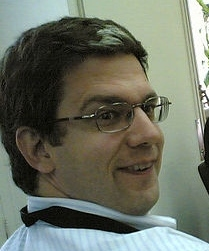
\includegraphics[width = 27 mm]{FTricas1.jpg},]
		\noindent  \emph{Fernando Tricas Garc\'{\i}a} es profesor
		titular de Lenguajes y Sistemas Inform\'aticos del Departamento
		de Inform\'atica e Ingenier\'{\i}a de Sistemas de la Universidad de
		Zaragoza.  Empez\'o a estudiar la blogosfera casi cuando a\'un no
		exist\'{\i}a (all\'a por el a\~no 2002) y a tratar de integrarla en los
		cursos y tareas docentes un poco despu\'es.  Ha impartido
		numerosas charlas relacionadas con el tema de la Web 2.0.
		Es actualmente Director de su departamento.  
		\end{window}}}

  \noindent que explicarle a nuestro interlocutor que las m\'aquinas virtuales
  que hab\'{\i}amos creado son computadoras diferentes aunque las vea en el
  mismo sitio? �Montamos un cl\'uster? �He o\'{\i}do mencionar a alg\'un nuevo
  proyecto de Internet de las Cosas (IoT) en la fila trasera? Y, si nos
  aburrimos, en la red podemos encontrar un mont\'on de proyectos que retar\'an
  nuestras diversas habilidades electr\'onicas e inform\'aticas. 
  Hemos dejado de lado (intencionadamente) Arduino y toda la familia de
  productos relacionada por tratarse de sistemas m\'as sencillos, no
  computadoras completas. Pero, desde luego, se trata tambi\'en de
  herramientas que deber\'{\i}an figurar en nuestros an\'alisis y ser tenidas en
  cuentas para los proyectos en los que encajen, pr\'acticamente en cualquier
  asignatura de Inform\'atica. Pero no queremos olvidar para terminar el
  aviso de que Raspberry Pi
 no es nuestra \'unica posibilidad. Como en casi
  todo, existen alternativas: BeagleBoard produce placas con
  funcionalidades similares desde hace bastante tiempo (algo m\'as caras),
  Intel ha entrado recientemente en este campo con el Edison. Y no podemos
  olvidarnos de la multitud de \textsl{sticks} USB con diversas versiones de
  Android, aunque en este caso la orientaci\'on suele ser claramente hacia el
  consumo multimedia. Y otras que veremos en el futuro m\'as cercano incluso
  m\'as baratas: por 9\$ la unidad, podr\'{\i}as tener un verdadero cluster de
  {\em C.H.I.P.s}.

  En resumen, hay vida fuera de los ordenadores de sobremesa, y los
  ordenadores, cuanto m\'as peque\~nos e incompletos, m\'as posibilidades tienen
  de creaci\'on de todo tipo de proyectos poco convencionales que mezclan la
  creatividad con la tecnolog\'{\i}a, en un verdadero esp\'{\i}ritu artesano. 
 \noindent 

\bigskip

\noindent\emph{Todas las columnas de la serie Docencia 2.0
pueden descargarse en formato LaTeX desde
{\small\url{https://github.com/ReVision-Docencia-20/Columnas}}}

\noindent\rule{90mm}{1pt}

{\small \noindent
\includegraphics[height = 4ex]{CC.png} 2015 JJ. Merelo, F. Tricas. Este art\'{\i}culo es de acceso libre distribuido bajo los t\'erminos
de la Licencia Creative Commons de Atribuci\'on, que permite copiar,
distribuir y comunicar p\'ublicamente la obra en cualquier medio, s\'olido
o electr\'onico, siempre que se acrediten a los autores y fuentes
originales}

\end{multicols}
\end{document}
